\documentclass[12pt]{article}
\usepackage{amsmath}
\usepackage{amssymb}
\usepackage{amsthm}
\usepackage{amsfonts}
\usepackage{algpseudocode}
\usepackage{algorithm}
\usepackage{mathrsfs}
\usepackage{graphicx}
\usepackage{times}
\usepackage{color}
\usepackage{appendix}
\usepackage{subfigure}
\usepackage{enumerate}
\usepackage{mathtools}
\usepackage{multirow}
\usepackage{booktabs}
\numberwithin{table}{section}
\usepackage{enumitem} %change list depth

\usepackage{listings}
\usepackage{xcolor}

\definecolor{codegreen}{rgb}{0,0.6,0}
\definecolor{codegray}{rgb}{0.5,0.5,0.5}
\definecolor{codepurple}{rgb}{0.58,0,0.82}
\definecolor{backcolour}{rgb}{0.95,0.95,0.92}

\lstdefinestyle{mystyle}{
	backgroundcolor=\color{backcolour},   
	commentstyle=\color{codegreen},
	keywordstyle=\color{magenta},
	numberstyle=\tiny\color{codegray},
	stringstyle=\color{codepurple},
	basicstyle=\ttfamily\footnotesize,
	breakatwhitespace=false,         
	breaklines=true,                 
	captionpos=b,                    
	keepspaces=true,                 
	numbers=left,                    
	numbersep=5pt,                  
	showspaces=false,                
	showstringspaces=false,
	showtabs=false,                  
	tabsize=2
}

\lstset{style=mystyle}

\usepackage{tikz}
\usetikzlibrary{positioning}
\usetikzlibrary{arrows,arrows.meta}
\setlistdepth{8}
\renewlist{itemize}{itemize}{8}

\newcommand{\question}[2][]{\begin{flushleft}
		\Large\textbf{Question #1}: \large\textit{#2}
		
\end{flushleft}}
\newcommand{\sol}{\textbf{Solution}:} %Use if you want a boldface solution line
\newcommand{\maketitletwo}[2][]{\begin{center}
		\Large{\textbf{Homework #1}
			
			ECE 590: Towards More Reliable Software} % Name of course here
		\vspace{5pt}
		
		\normalsize{Jeff Fan  \hspace{1em} $\left|\right|$ \hspace{1em}zf70@duke.edu  % Your name here
			
			\today}        % Change to due date if preferred
		\vspace{15pt}
		
\end{center}}

\begin{document}
	\maketitletwo[1]  % Optional argument is assignment number
	%Keep a blank space between maketitletwo and \question[1]
	
\section*{Question 1: } 

\textbf{a. List all the attributes of software dependability and explain their meanings.}

\textbf{Availability:} This refers to the readiness of a system for correct service. It focuses on ensuring that the system is accessible and usable when needed.

\textbf{Reliability:} This attribute is concerned with the continuity of correct service. It measures how consistently a system performs its intended function without failure over time.

\textbf{Safety:} Safety is the attribute that emphasizes the absence of catastrophic consequences on the users and the environment. It's about ensuring that the system does not cause harm or adverse effects.

\textbf{Integrity:} This pertains to the absence of improper system alterations. Integrity ensures that the system's data and operation are not unlawfully or erroneously modified or tampered with.

\textbf{Maintainability:} This is the ability of the system to undergo modifications and repairs. Maintainability makes it easier to update, improve, and fix the system as needed.
	
\textbf{Confidentiality:} This is defined as the absence of unauthorized disclosure of information. It's crucial for protecting sensitive information from unauthorized access or exposure.\\
\\
\textbf{b. Which do you think is the best means to achieve software dependability in the above paper and why? }

In my view, I consider fault tolerance as the best means to achieve software dependability based on the content of the paper. Fault tolerance is primarily aimed at failure avoidance, meaning it allows a system to continue operating correctly even in the presence of faults. This is crucial for systems where high availability and reliability are non-negotiable, such as in critical infrastructure systems or financial services. It also includes a range of techniques like error detection, system recovery, rollback, rollforward, and compensation. These methods ensure that not only are errors detected, but the system can also recover from them, thus maintaining service continuity. 

Fault tolerance techniques often include the concept of error confinement areas, which help in localizing the impact of a fault. Additionally, the effectiveness of a fault tolerance technique is measured by its coverage, or how well it can handle a range of fault scenarios. While fault tolerance is effective on its own, it also complements other dependability strategies like fault prevention, removal, and forecasting. This interplay enhances overall system dependability, making fault tolerance a key component in a comprehensive dependability strategy.\\
\\
\textbf{c. Use your own words to describe the different definitions of fault, error and failure.}

Fault: Imagine a fault as a weak link in a chain. It's a defect or flaw within the system, but it hasn't yet caused a problem. The chain is still holding together, but the weak link represents a potential point of failure. In technical terms, a fault is a defect in a system's hardware, software, or design that has the potential to cause an error. It's like a dormant seed that, under the right conditions, can sprout into a bigger issue.

Error: Using the chain analogy, an error occurs when the weak link starts to give way under stress. The chain hasn't broken yet, but there's a clear sign that something is wrong – the link is deforming or starting to crack. In the context of computing systems, an error is the manifestation of a fault. It's a deviation from the correct or expected behavior of the system. The system hasn't failed yet, but there's an incorrect state within it, like corrupted data or a malfunctioning process.

Failure: Finally, a failure happens when the weak link in the chain breaks, causing the entire chain to fail in its function of holding something together. In a computing system, a failure is the point at which the system can no longer deliver the expected service to the user. It's the observable consequence of an error, where the system's operation deviates from what's expected, like a system crash or incorrect output.

To sum up, a fault is like a weak link in a chain – a potential problem; an error is like the weak link starting to give way – a problem in progress; a failure is like the chain breaking due to the weak link – a complete breakdown in operation.

\section*{Question 2: } 

\textbf{Take any program that you have written and identify at least one fault (bug), the errors it will cause, the inputs that will trigger the fault and failure that results. How can you avoid them next time?}

\begin{lstlisting}[language=Java]
	import java.io.*;
	import java.net.ServerSocket;
	import java.net.Socket;
	import java.lang.reflect.Method;
	
	public class SocketServer {
		public static void main(String[] args) throws Exception {
			ServerSocket serverSocket = new ServerSocket(8080);
			System.out.println("Server started. Listening on port 8080...");
			
			while (true) {
				try (Socket clientSocket = serverSocket.accept();
				BufferedReader in = new BufferedReader(new InputStreamReader(clientSocket.getInputStream()));
				PrintWriter out = new PrintWriter(clientSocket.getOutputStream(), true);) {
					
					String inputLine = in.readLine();
					Method method = SocketServer.class.getMethod(inputLine);
					String response = (String) method.invoke(null);
					out.println(response);
				} catch (Exception e) {
					e.printStackTrace();
				}
			}
		}
		
		public static String getTime() {
			return "The current time is " + System.currentTimeMillis();
		}
	}
\end{lstlisting} 

\textbf{Fault:} The potential fault in this program is the lack of validation of the input line (line 17), which is used directly to reflectively call a method. If the input does not correspond to a method name, or if it is a method name not intended to be called, this could lead to errors.

\textbf{Error:} The primary error this fault can cause is a \textbf{NoSuchMethodException} if an input string is received that doesn't correspond to any method in the class. Additionally, if the input is malicious, it could potentially call unintended methods (if they exist and are public and static), leading to security vulnerabilities.

\textbf{Trigger Inputs:} Any input string that is not exactly "getTime" will trigger the fault. For example, inputs like "gettime", "Time", or "randomString" will cause the program to throw an exception.

\textbf{Failure: }The failure resulting from this error would be the server crashing or behaving unexpectedly, potentially exposing the system to security risks. The server might also respond with an error message or stack trace to the client, which is undesirable in a production environment.\\

\textbf{How to Avoid: } 

a. Always validate user inputs, especially when using them in sensitive operations like reflection. In this case, a whitelist of allowed method names could be used to validate the input before attempting to invoke a method.

b. We can enhance the error handling by specifically catching NoSuchMethodException and returning a user-friendly message. For example
\begin{lstlisting}[language=Java]
	...
			Set<String> allowedMethods = Set.of("getTime");
			while (true) {
				try (Socket clientSocket = serverSocket.accept();
				BufferedReader in = new BufferedReader(new InputStreamReader(clientSocket.getInputStream()));
				PrintWriter out = new PrintWriter(clientSocket.getOutputStream(), true);) {
					
					String inputLine = in.readLine();
					try {
						if (allowedMethods.contains(inputLine)) {
							Method method = SocketServer.class.getMethod(inputLine);
							String response = (String) method.invoke(null);
							out.println(response);
						} else {
							out.println("Invalid method request.");
						}
					} catch (NoSuchMethodException e) {
						out.println("Requested method not found.");
					} catch (Exception e) {
						out.println("An error occurred.");
						e.printStackTrace(); // For debugging purposes
					}
	...
	
\end{lstlisting} 

c. We can also restrict the use of reflection as it can be a security risk. If reflection is necessary, ensure it's tightly controlled and secure. Employ principles like least privilege and secure coding practices.

d. We can implement proper logging to record unusual activities or inputs. Monitoring these logs can help in quickly identifying and rectifying issues.

\section*{Question 3: } 

\textbf{Find a well-publicized incident, read about it and determine, the fault(s), errors and failure of this accident. And find out how the engineers react after the incident happens?}

The Target data[1] breach of 2013 is a famous example of a cybersecurity incident.

\textbf{Faults:} 
The initial fault lay in the security systems of both Target and its third-party vendor, Fazio Mechanical. The vendor's lack of malware detection software and the failure of both companies to properly segment their networks created vulnerabilities.

\textbf{Errors:}
The errors occurred when cybercriminals successfully executed a phishing scam to gain network access, installed malware on Target's point-of-sale systems, and began collecting customer data. The malware's presence was detected, but Target initially failed to act on these alerts.

\textbf{Failure:}
The failure was the large-scale compromise of approximately 40 million customers' credit/debit card information and 70 million customers' personal details (e.g., names, addresses, phone numbers), resulting in significant financial and reputational damage to Target.

\textbf{Engineers' Response:}
Post-breach, Target undertook several recovery steps including working with a forensics firm, offering credit monitoring to customers, upgrading their point-of-sale systems, and implementing better network segmentation and access controls. They faced over 140 lawsuits, an \$18.5 million settlement, and changes in executive leadership due to the breach.\\

{\small [1] target investigating data breach. https://krebsonsecurity.com/2013/12/sources-target-investigating-data-breach/}

\section*{Question 4: } 
\textbf{Develop and describe a classification of errors.}
\\
\textbf{1. System-Level Errors}

\textbf{Hardware Failures:} Malfunctions in physical components of the system, like hard drive crashes or memory corruption.

\textbf{Operating System Errors:} Issues within the operating system that affect software execution, such as file system errors or driver conflicts.
\\
\textbf{2. Application-Level Errors}

\textbf{Runtime Exceptions:} Errors that occur during the execution of an application, like null pointer exceptions or out-of-bounds errors.

\textbf{Logic Errors:} Flaws in the application's logic leading to incorrect behavior or results, even though the program runs without crashing.

\textbf{Data Processing Errors:} Issues in handling and processing data, such as incorrect data parsing or arithmetic errors.

\textbf{Concurrency Issues:} Problems arising in multi-threaded applications, like race conditions or deadlocks.

\textbf{Resource Leaks:} Inadequate management of resources leading to issues like memory leaks or file descriptor exhaustion.
\\
\textbf{3. Interface-Level Errors}

\textbf{API Misuse:} Incorrect use of APIs or failure to handle API errors gracefully.

\textbf{Integration Problems:} Issues arising when integrating with other software components, services, or databases.

\textbf{Network Communication Errors:} Problems in the network layer, such as failure to handle lost connectivity or delayed responses.
\\
\textbf{4. User Interface-Level Errors}

\textbf{Input Validation Errors: } Failure to properly validate user inputs leading to incorrect or unexpected behavior.

\textbf{Navigation Flaws:} Issues in the UI flow that confuse users or lead them to dead ends.

\textbf{Display Issues:} Problems with how information is presented on the screen, like overlapping text or incorrect data representation.
\\
\textbf{5. Configuration-Level Errors}

\textbf{Setup and Configuration Mistakes:} Errors due to incorrect setup or configuration parameters of the software or its environment.

\textbf{Dependency Issues:} Problems arising from incompatible or missing software dependencies.
\\
\textbf{6. Security-Level Errors}

\textbf{Vulnerabilities:} Flaws that compromise the security of the application, like buffer overflows or SQL injection vulnerabilities.

\textbf{Access Control Issues:} Problems related to authentication and authorization, like privilege escalation or unauthorized access.
\\
\textbf{7. Development and Build-Level Errors}

\textbf{Compilation Errors:} Issues that prevent the source code from successfully compiling, like syntax errors or unresolved references.

\textbf{Build and Deployment Mistakes:} Errors in the build pipeline or deployment process, leading to incorrect or failed deployments.\\

Here I draw the figure to clearly show you the classification:
\\
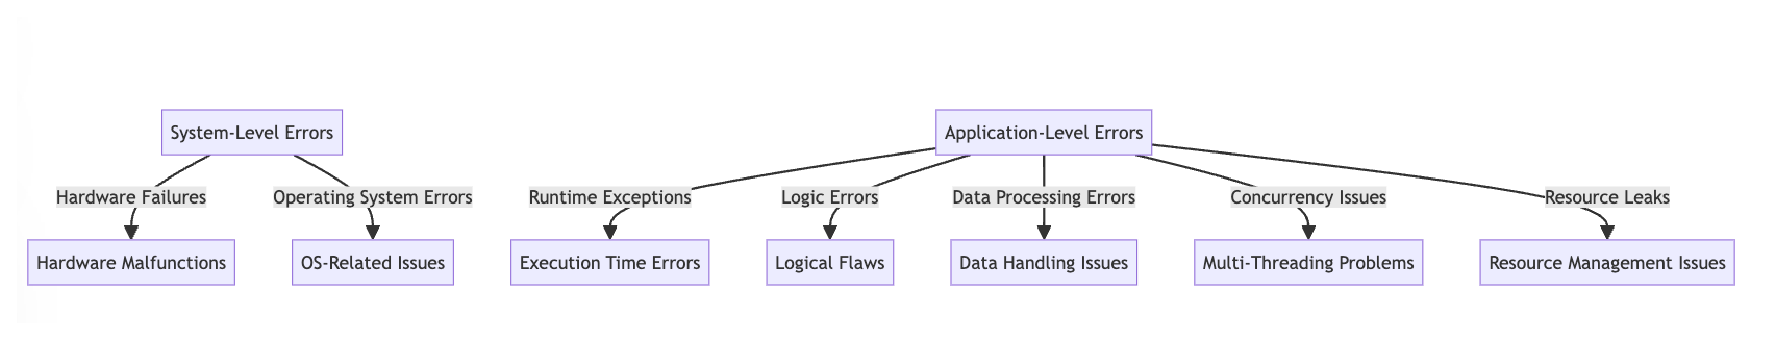
\includegraphics[width=1.2\textwidth]{1.eps}
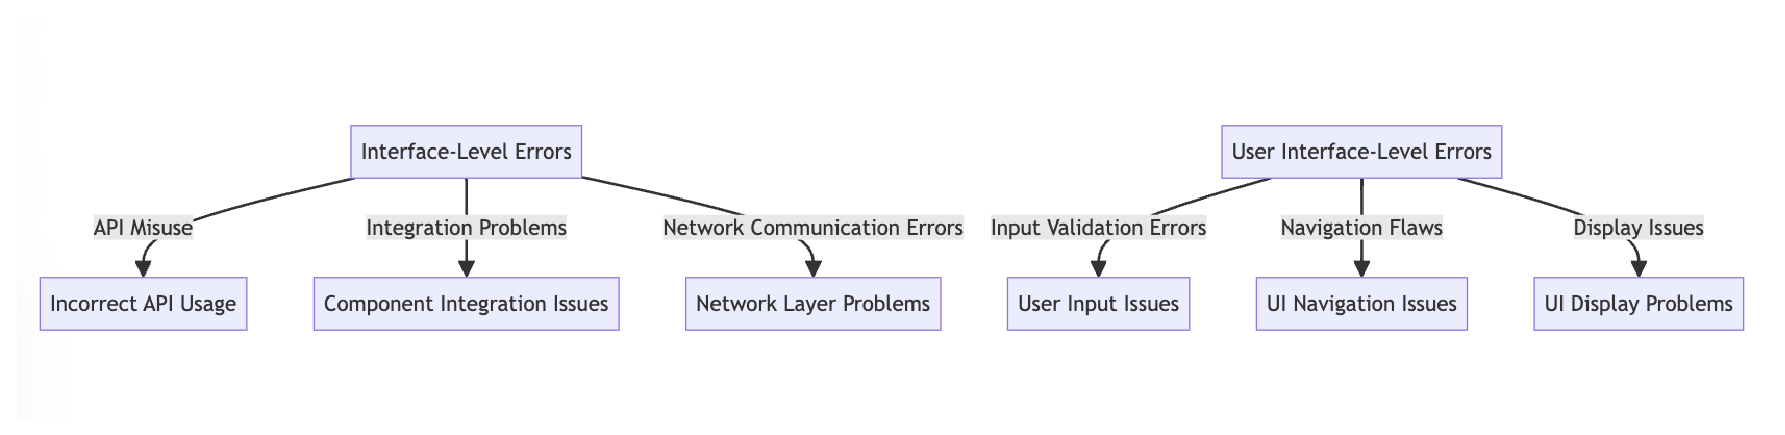
\includegraphics[width=1.2\textwidth]{2.eps}
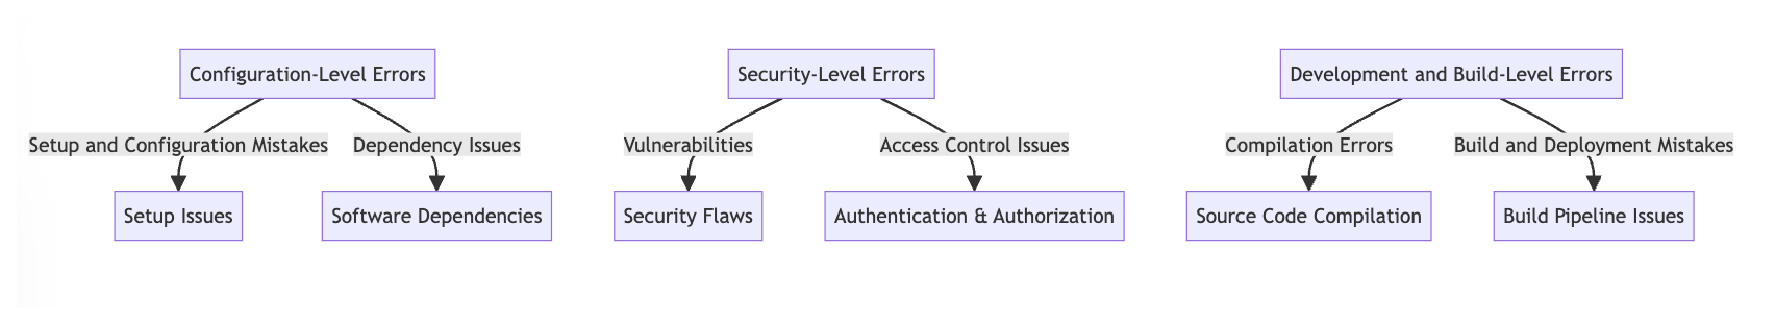
\includegraphics[width=1.2\textwidth]{3.eps}


\end{document}
